\section{Vue générale}

\begin{figure}[h]
\begin{center}
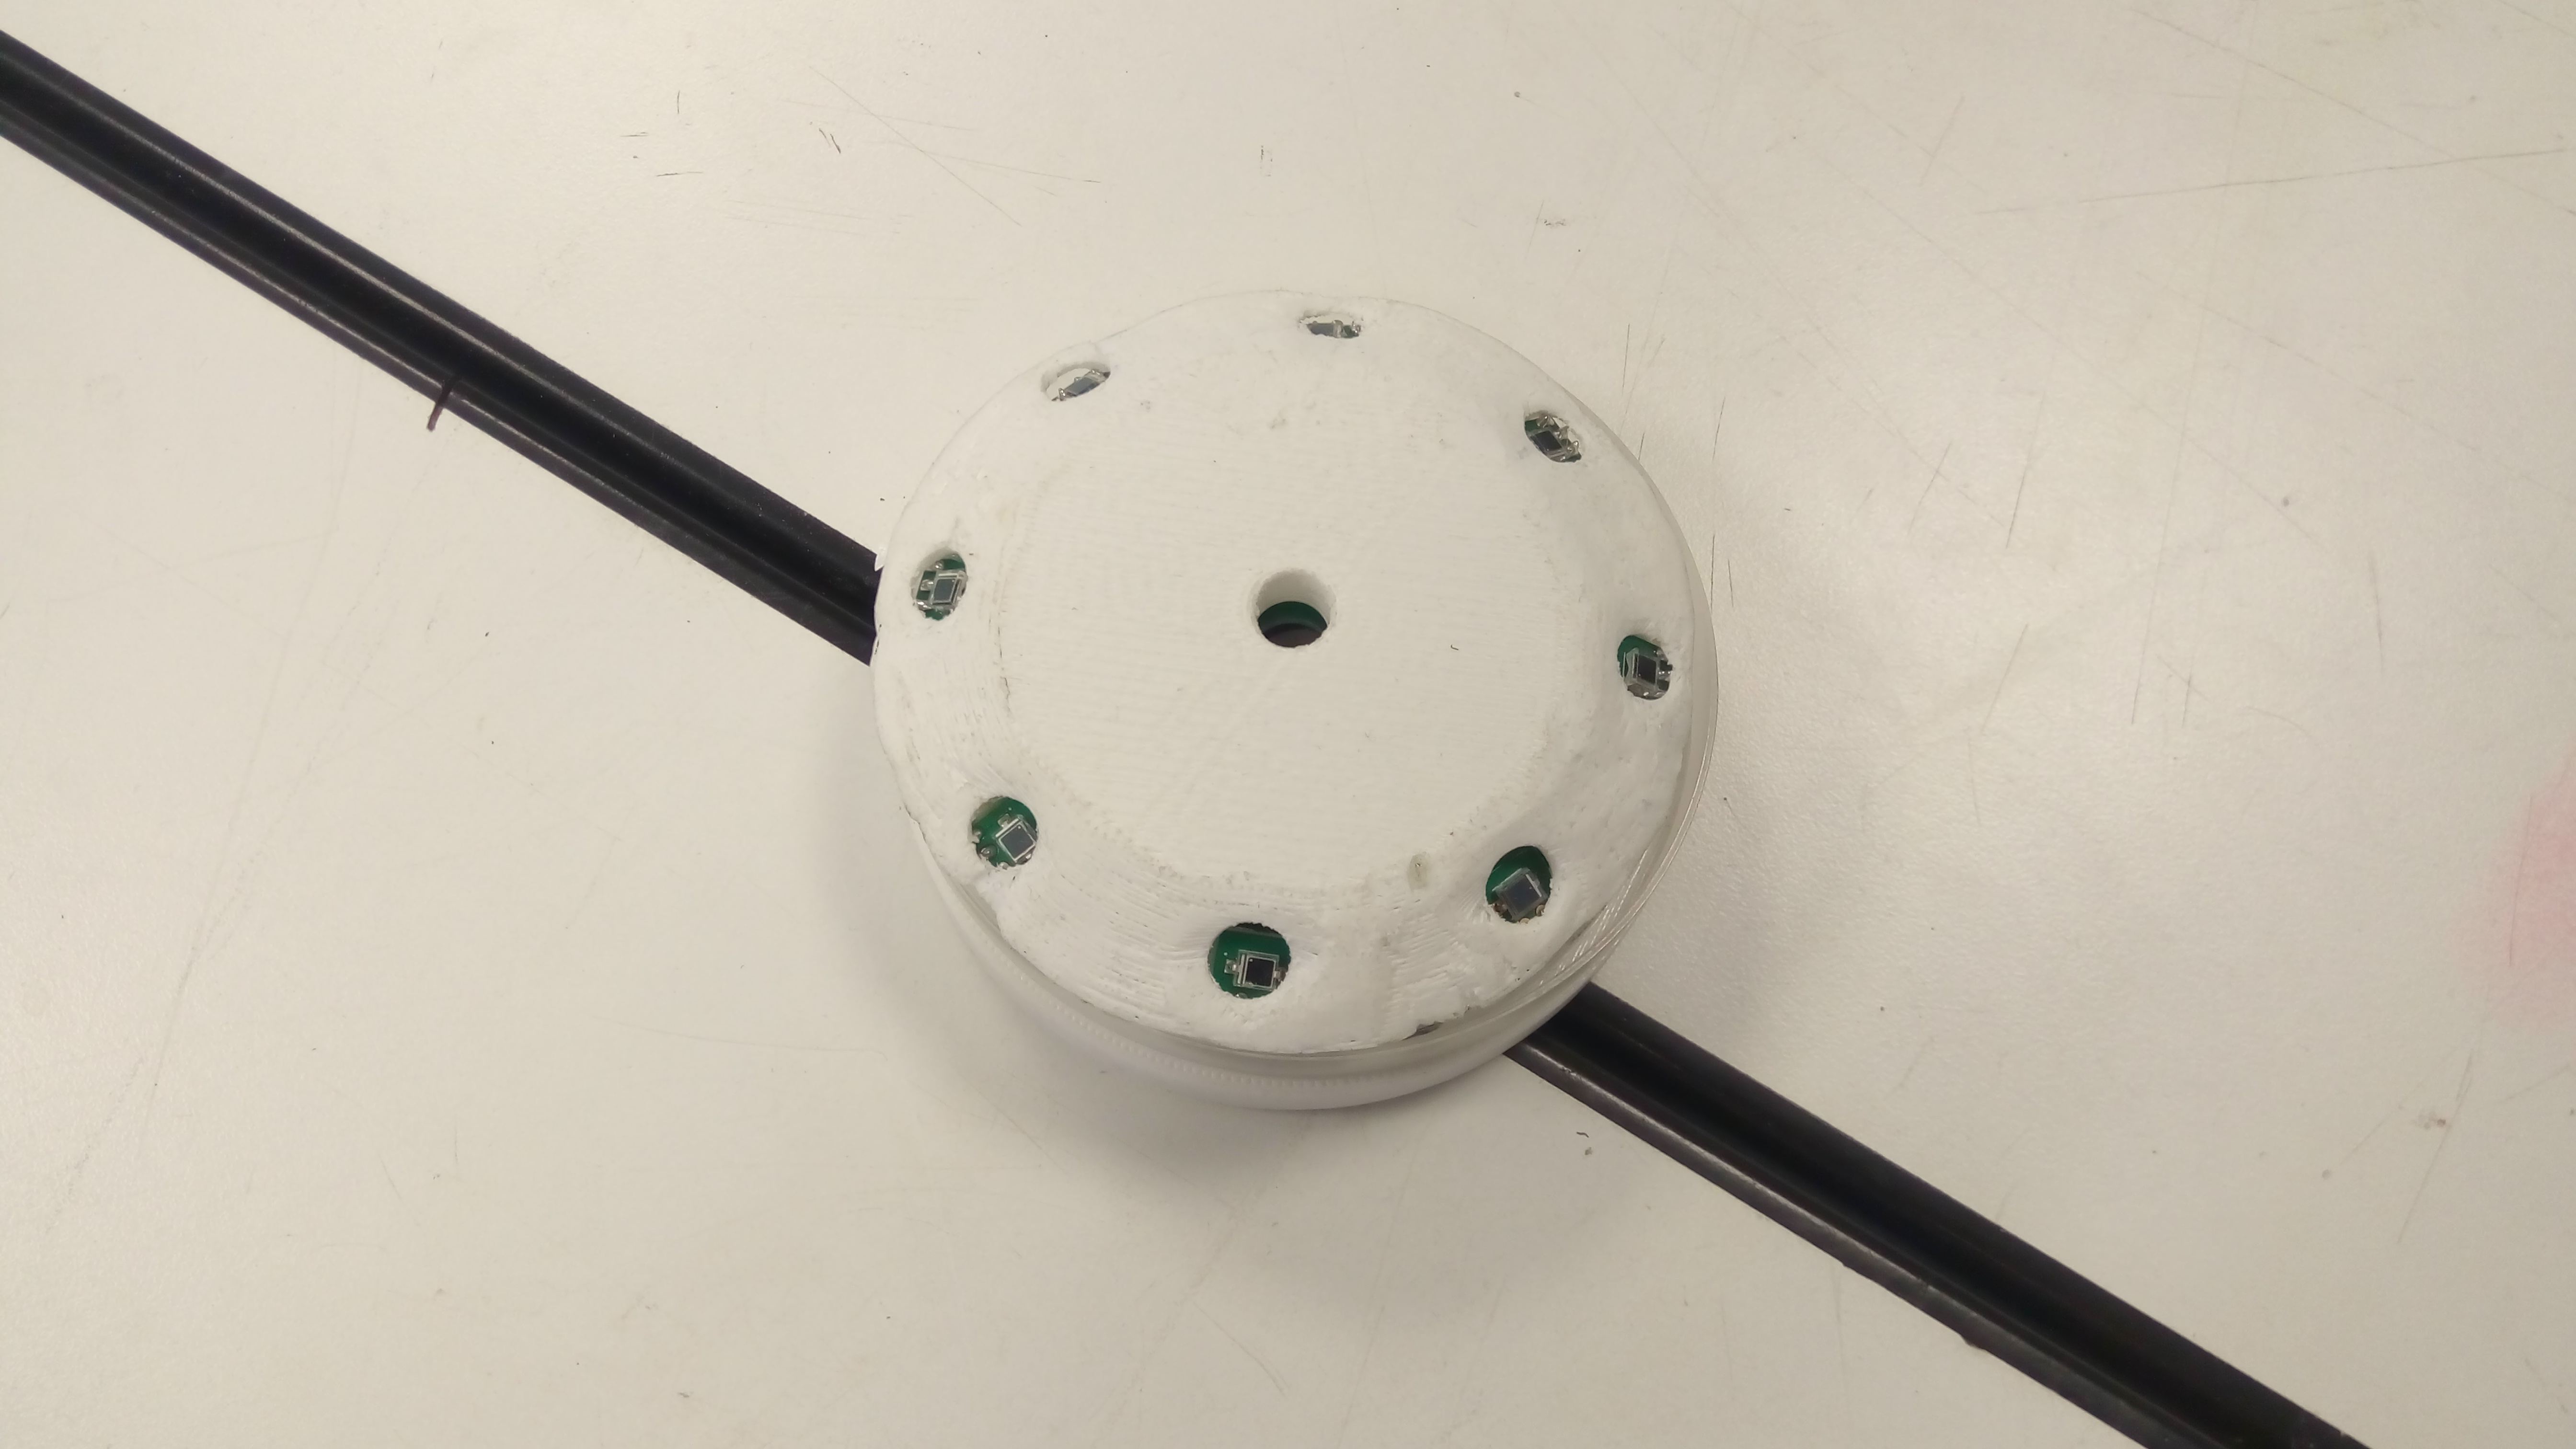
\includegraphics[scale=0.05]{imgs/IMG_20180525_120520.jpg}
\end{center}
\caption{Un tracker Vive.}
\end{figure}

De l'extérieur, un tracker Vive se présente sous la forme d'un cylindre large et plat, avec des cratères inclinés sur le dessus. Sur le dessus, nous pouvons apercevoir 8 photodiodes sensibles à la lumière infrarouge, ce sont les capteurs. Sur la tranche, une bande de LEDs de type Neopixel est installé à des fins de débug et d'information. Enfin, sur le dessous, un port USB permet de récupérer les données sur un PC.

N.B. : Un tracker Vive ressemble beaucoup à un générateur ARK de Iron-man. Cette ressemblance n'est que fortuite.

\section{Architecture électronique}

Un tracker Vive est composé de 8 cartes IRInterface, dédié au prétraitement et à la conversion analogique - numérique des impulsions vive, et d'une carte IRoise (notez le jeu de mots), dédié au calcul de positionnement et aux différentes communications.

\begin{figure}[h]
\begin{center}
\includegraphics[scale=0.2]{imgs/DSC01093.jpg}
\end{center}
\caption{Les différentes cartes électroniques développées. La carte IRoise (au centre) et les cartes IRInterfaces (autour) sont au coeur du tracker.}
\end{figure}

\subsection{Les cartes IRInterface}

Les cartes IRInterfaces ont été créés dans le but de filtrer les bruits / parasites sur le signal IR fourni par les lasers. Pour cela, la photodiode IR (une BPW34) n'est sensible que dans une bande de longueur d'onde : de 500 à 1000nm avec un pic de sensibilité au alentour des 950nm.

De plus, un circuit intégré, le TS4231, filtre les perturbations à 50-60Hz dû aux ampoules à incandescence et aux tubes fluorescents (ou "`néons"'). Il rejette aussi tout signal non modulé à une fréquence porteuse comprise entre 1Mhz et 10Mhz. Les lasers des balises "`Lighthouse"' de première génération (celle disponibles au BDI) est d'environ 2Mhz (1.8Mhz pour être précis). Le TS4231 est capable de fournir un signal d'enveloppe, c'est celui qui nous intéresse dans un premier temps, sur la patte ENVELOPPE mais aussi de fournir un signal numérique carré, image de la fréquence porteuse du signal sur la patte DATA. Ces deux signaux sont envoyés à la carte IRoise.

% Images IRInterface (LED d'un coté, triad de l'autre)

\subsection{Les cartes IRoise}

Les cartes IRoise sont équipés d'un PSoC (Programmable System-On-Chip, marque déposée de Cypress Semiconductors) afin de réaliser les mesure de timing et donc d'angle et, par conséquent, de recalculer la position de la balise. Elles sont aussi équipées d'une centrale inertielle 9 axes, le MPU-9250, afin de pouvoir interpoler entre les mesures Vive, si jamais le tracker ne reçoit plus de lumière des balises "`Lighthouse"'.

Différents connecteurs sont présents pour permettre un branchement (relativement) aisée des différents éléments du tracker à savoir : les cartes IRInterfaces, la bande de Neopixel, le xBee, le câble USB et éventuellement le programmeur PSoC pour flasher le tracker. Une rangée de picots est placé à des fins de configuration rapide via jumpers et peut servir à étendre les fonctionnalités de la carte.

% Images IRoise, avec et sans les différents composants

